\documentclass[journal, 12pt, onecolumn, draftclsnofoot]{IEEEtran}
% \documentclass[10pt,conference]{IEEEtran} %INFOCOM 20'
\usepackage{extarrows}
\usepackage[linesnumbered,vlined,ruled]{algorithm2e}
\usepackage{algorithmic}
\usepackage{etoolbox}
\usepackage{cite}
% \usepackage[noend]{algpseudocode}
\usepackage{graphicx}
\graphicspath{ {./images/} }
\usepackage{amsmath,amsthm,amssymb,amsfonts,mathrsfs}
\usepackage{mathtools}
\usepackage[dvipsnames]{xcolor}
\usepackage{dcolumn}
\usepackage[utf8]{inputenc}
\usepackage{soul}
\usepackage{array}
\usepackage{tabulary}
\usepackage{enumitem}

\newcommand{\revise}{\color{black}}
\newcommand{\revisesec}{\color{blue}}
\newcommand{\fixit}[1]{{\leavevmode\color{red}(#1)}}
\newcommand{\comments}[1]{{\leavevmode\color{blue}#1}}
\newcommand{\deny}[1]{}
\newcommand{\needref}[1]{\text{[#1]}}
%---------------------------------------------------------------%
\newcommand{\eq}{=}
\newcommand{\domZ}{\mathbb{Z}_{*}}
\newcommand{\domP}{\mathbb{Z}_{*}}
\newcommand{\Expect}{\mathbb{E}}
\newcommand{\vecOne}{\mathbf{1}}
\newcommand{\ind}{\mathbf{I}}
\newcommand{\mat}{\mathbf}
\newcommand{\Poisson}{\text{Poisson}}
\newcommand{\Bernoulli}{\text{Bernoulli}}
\newcommand{\define}{\triangleq}
\newcommand{\leadto}{\Rightarrow}
\newcommand{\vecG}{\boldsymbol}
\renewcommand{\vec}{\mathbf}
\DeclarePairedDelimiter{\set}{\{}{\}}
\DeclarePairedDelimiter{\norm}{|}{|}
\DeclarePairedDelimiter{\Inorm}{\|}{\|_1}
\DeclarePairedDelimiter{\Paren}{\bigg(}{\bigg)}
\DeclarePairedDelimiter{\Bracket}{\bigg[}{\bigg]}
\DeclarePairedDelimiter{\Brace}{\bigg\{}{\bigg\}}
%---------------------------------------------------------------%
\newcommand{\Stat}{\mathbf{S}}
\newcommand{\Policy}{\vecG{\Omega}}
%---------------------------------------------------------------%
\newtheorem{Definition}{Definition}
\newtheorem{Problem}{Problem}
\newtheorem{Lemma}{Lemma}
\newtheorem{Theorem}{Theorem}
\newtheorem{Algorithm}{Algorithm}
\newtheorem{Scheme}{Scheme}
\newtheorem{Scenario}{Scenario}
\newtheorem{Assumption}{Assumption}
\newtheorem{Proposition}{Proposition}
\newtheorem{Remark}{Remark}
\newtheorem{Solution}{Solution}
\newtheorem{Baseline}{Baseline}
\newtheorem{Example}{Example}
\newtheorem{Corollary}{Corollary}
\newtheorem{Model}{Model}

\begin{document}
	
	\title{
		Joint Resource Scheduling for \deny{Heterogeneous} Communication and Computation Tasks in 5G C-RAN
	}
	\author{
        \IEEEauthorblockN{
            Yifei Sun,
            Yuncong Hong%,
            % Rui Wang,
            % Haisheng Tan,
            % Francis C.M. Lau
        }
        % \IEEEauthorblockA{\IEEEauthorrefmark{1}
        %     Department of Electrical and Electronic Engineering, Southern University of Science and Technology, Shenzhen, China \\
        % }
        % \IEEEauthorblockA{\IEEEauthorrefmark{2}
        %     Department of Computer Science, The University of Hong Kong, Hong Kong, China \\
        % }
        % \IEEEauthorblockA{\IEEEauthorrefmark{3}
        %     LINKE Lab, University of Science and Technology of China, Hefei, China \\
        % }
    }%
	\maketitle

	% \begin{abstract}
    In this paper, we consider a MEC scenario with C-RAN architecture,
    %Based on network function virtualization (NFV), 
    where the communication data processing tasks (DTs) and general computation tasks (CTs) can be implemented by virtual BBUs (vBBUs) and virtual MEC servers (vMESs) on general-purposed processors, respectively.
\end{abstract}
	\section{Introduction}
\label{sec:intro}
\comments{
    C-RAN is the future in 5G.
    The functions of base station (eNB) are splitted into remote radio head (RRH) and Baseband Unit (BBU).
    It is preffered to be implemented in a centralized and virtualized manner.
}

\comments{
    \textbf{Motivations.}
    a) virtualization of C-RAN on general-purpose processors (GPPs) together with MEC is better than no virtualization, which benefits from energy saving, and network simplicity \cite{cran-survey};
    b) jointly dynamic computation resource allocation for BBU and MEC;
    c) There does not exist trivial/heuristic algorithm to do the joint scheduling on communication and computation resource?
}

In this paper, we propose a novel framework where both BBU tasks and general edge computing tasks are processed simultaneously in a homogeneous edge cloud with general-purposed processors.
Our major contributions in this new optimization scenario are summarized as follows.
\begin{itemize}
    \item We propose a joint computation resource allocation scheme under MDP framework;
    \item We propose the parameterized computation model for BBU functions on general purpose processor, and carry out experiments to examine the parameter fitness;
    \item The performance bound of our proposed algorithm is proved.
\end{itemize}

\begin{figure*}[htb!]
    \centering
    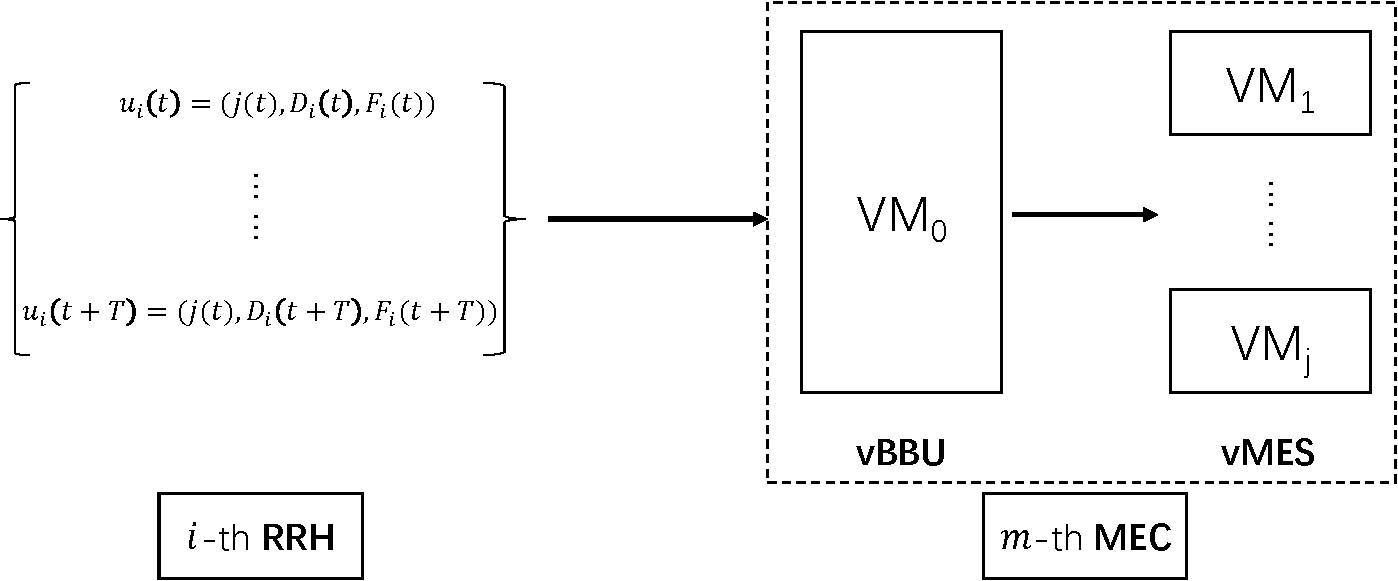
\includegraphics[width=0.9\textwidth]{images/cran-system-model.pdf}
    \caption{The Illustration of System Model.}
    \label{fig:system-model}
\end{figure*}
	\section{Background}
\label{sec:related}

\subsection{C-RAN Functional Split}
\comments{
    (Simply elaborate how and why we take such C-RAN implementation in 5G specification suggestion)
}

\subsection{Related Works}
%NOTE: MEC scheduling works
\comments{
    With the prosperity of large scale big data and computation intensive applications, mobile edge computing (MEC) is proposed to perform more real-time tasks than cloud computing \cite{mec-a1}.
    Edge computing aims at placing the computation task closer to user equipment (UE) and hence alleviate the communication overhead.
}

% There are several works considering but with simple CPU per cycles (CPS) consumption to evaluate the performance.
% In \cite{mec-b1}, the authors considered a mobile-edge computation offloading (MECO) system, both with local and edge computing.
% In \cite{mec-b1}, 
% In \cite{mec-b2}, 
% In \cite{mec-b3}, 
% In \cite{mec-b4}, 

%NOTE: vBBU study on channel multiplexing
% In \cite{cran-sim-PIMRC13}, the authors consider the signal processing of RRH offloading to the pooled baseband resource (vBBU), and analyzed the multiplexing gain by performing a simulation. The authors proposed a computation resource model whose Giga-Operations Per Second (GOPS) could scale with load and transmission mode. %each cell supports three sectors (three hexagonal area)

%NOTE: joint vBBU and vMEC scheduling
    
	% \input{src/02b-motivation.tex}
	\section{System Model}
\label{sec:model}

%-----------------------------------------------------------------------------------------%
\subsection{BBU Functional Split}
\comments{
    (Simply elaborate how and why we take such C-RAN implementation in 5G specification suggestion)
}

%-----------------------------------------------------------------------------------------%
\subsection{Network Model}
There are $K$ RRHs and $M$ edge clouds considered in our network which are denoted as $\mathcal{K}=\set{1,\dots,K}$ and $\mathcal{M}=\set{1,\dots,M}$, respectively.
Each RRH servers the mobile devices (MDs) in a disjoint coverage from other RRHs which is denoted as $\mathcal{C}_{k}$, and has a fronthaul link to one edge cloud for further signal and data processing.
% Furthermore, we assume that each edge cloud is deployed in a Function-as-a-Service (FaaS) manner, where \comments{no constantly running server processes are required}.
As illustrated in Fig.\ref{fig:system-model}, a set of virtual machines (VMs) are deployed in each edge cloud which is consist of the VM for baseband unit (BBU) functions (VMB) and the VMs for other computation tasks (VMC).
It's assumed that there are fixed $J$ types of computation tasks supported in the edge cloud which is denoted as $\mathcal{J}=\set{1,\dots,J}$ and the VM for the type-$j$ job in the $m$-th edge cloud is denoted as $V_{m,j}$.
Specifically, there is one and only one VM for BBU functions which is denoted as $V_{m,0}$ ($\forall m\in\mathcal{M},j\in\mathcal{J}$).
% A set of \emph{function handlers} (FHs) are deployed in each edge cloud which includes the FH $V_{0}$ for functions of Baseband Unit (BBU) and the FHs for other $J$ types of computation tasks which are denoted as $V_{j}$ ($\forall j\in\set{1,\dots,J}$).

% The time axis of dispatching is organized by time slots.
The system is scheduled at the minimum time unit called \emph{frame}.
We only consider the active mobile devices in the system, which is in data transmission or waiting for data processing in the edge cloud.
At the $t$-th frame, the $k$-th RRH would serve a set of \comments{active MDs} in the region $\mathcal{C}_{k}$, which is denoted as $\mathcal{U}_{k}(t)$ ($\forall k\in\mathcal{K}$).
At each frame, there would be at most one MD in the region $\mathcal{C}_{k}$ being selected for data transmission via the $k$-th RRH to one edge cloud for further data processing.
The uploaded data would be categorized into two kinds of tasks uploaded from users: baseband/basic task (BT) and computation task (CT).
A BT is completed after VMB processing and needs no VMC processing, whose average arrival rate is denoted as $\lambda_{k,0}$ in the region $\mathcal{C}_{k}$;
a type-$j$ CT requires tandem processing of VMB and the corresponding VMC, whose average arrival rate is denotes as $\lambda_{k,j}$ in the region $\mathcal{C}_{k}$ ($\forall k\in\mathcal{K}, j\in\mathcal{J}$).
Futhermore, the status of the $n$-th task (BT or CT) in the region $\mathcal{C}_{k}$ in the $t$-th frame is denoted as follows.
\begin{align}
    u_{n,k}(t) \define \Paren{
        \tilde{t}_{n}, \tilde{j}_{n}, \tilde{m}_{n}, \tilde{d}_{n}, D_{i,k}(t), F_{i,k}(t)
    },
\end{align}%
where:
\begin{itemize}
    \item $\tilde{t}_{n}, \tilde{j}_{n}, \tilde{m}_{n}, \tilde{d}_{n}$ denotes the appearing time, job type, index of dispatched edge cloud and input data size (with the unit as bit) for the $n$-th task, respectively ($\tilde{j}_{n}\in\set{0}\cup\mathcal{J}$, $\tilde{m}_{n}\in\mathcal{M}$); $\tilde{d}_{n}$ follows uniform distribution between $d_{\tilde{j}_n,\min}$ and $d_{\tilde{j}_n,\max}$ ($\forall n \in \set{1, \dots, |\mathcal{U}_{k}(t)|}$);
    \item $D_{i,k}(t)$ denotes the remaining number of bits waiting for uploading;
    \item $F_{i,k}(t)$ denotes the remaining computation time on VMC.
\end{itemize}
Specifically, the computation time for type-$0$ job (i.e., a data task) has $F_{i}(t)=0$ ($\forall t$).
% We use the concept, \emph{active devices}, to name the mobile devices with computation tasks.
% In each frame, there is at most one active mobile device appears in each cell with probability $P_{i}^{\mathrm{N}}$. And the probability that an active device arrived in region $\mathcal{C}'$ is
% \begin{align}
% 	\mathrm{Pr}[\text{New active device in region }\mathcal{C}']=\int_{\mathcal{C}'}\lambda(\mathbf{l})ds(\mathbf{l}),\forall \mathcal{C}'\subset\mathcal{C}_{i}.
% \end{align}
% where $\lambda(\mathbf{l})$ is the probability density of the active device arrived in arbitrary location in the cell region $\mathbf{l}\in\mathcal{C}_{i}$ and $\int_{\mathcal{C}_{i}}\lambda(\mathbf{l})ds(\mathbf{l})=1$.
% It is assumed that the location of each active device is quasi-static during the period from it arrives to it completes the uplink transmission of the whole task. The active device becomes \textit{inactive} once the edge cloud finishes computing the whole task. Moreover, due to the small data size of the computation output, the downlink latency of the computation output is ignored.
% Let $\mathcal{U}_{i}(t)$ be the set of active devices in the $i$-th cell in $t$-th frame, $\mathcal{D}_{i}(t)\subset\mathcal{U}_{i}(t)$ be the subsets of the active devices whose tasks are just accomplished at the edge cloud in the $t$-th frame, and $n_{i,t}$ be the index of the new active device in the $i$-th cell arrived at the beginning of the $t$-the frame. Therefore, every active device is assigned with a unique index associated with the cell index and frame index it arrived.

%NOTE: How to upload, and how to evaluate VMB
Let $\rho^{\mathrm{Tr}}_{k, n}(t)$ denote the indicator for whether the $n$-th task in the $k$-th cell is being selected for uploading or not, and $\vecG{\rho}^{\mathrm{Tr}}(t) \define \set{\rho^{\mathrm{Tr}}_{k, n}(t) | \forall k\in\mathcal{K},n\in\set{1,\dots,|\mathcal{U}_{k}(t)|}}$ denote .
We assume that the MD and RRH are equipped with one antenna and $L$ antennas, respectively.
The signal-to-interference-plus-noise ratio (SINR) and transmission rate $r_{k,n}(t)$ between the $k$-RRH and the $n$-th user in the region $\mathcal{C}_{k}$ are denoted as follows.
\begin{align}
    \gamma_{n}(t) = \frac{
        \vecG{\theta}_{k,n}(t) \Inorm{h_{k,n,n'}(t)}^2
    }{
        \sum_{n' \neq n} \vecG{\theta}_{k,n}(t) \Inorm{h_{k,n,n'}(t)}^2 + \sigma_{i}^{2}
    }
    % \gamma_{k}(t)=\frac{p_{i,k}^{\mathrm{Tr}}(t)\rho_{i,i,k}|h_{i,i,k}(t)|^2}{\sum_{(j,m)\neq (i,k)}p_{j,m}^{\mathrm{Tr}}\rho_{i,j,m}|h_{i,j,m}(t)|^{2}+\sigma_{i}^{2}},
    \\
    r_{k}(t)= W\cdot \text{log}(1+\gamma_{k}(t)),
\end{align}%
where $W$ is the pre-allocated bandwidth (with the unit as Hz).
\fixit{
    The dynamics of the $k$-th transmission queue is given by
    \begin{align}
        Q_{k}^{\mathrm{Tr}}(t+1)=(Q_{k}^{\mathrm{Tr}}(t)-D_{k}^{\mathrm{Tr}}(t))^{+}
    \end{align}
    where $D_{k}^{\mathrm{Tr}}(t)=T_{\mathrm{f}}r_{k}(t)$.
}
% Let ${U}_{i}(t)$ denote the existing tasks in the $i$-th cell in the $t$-th frame
% \begin{align}
%     \mathcal{U}_{i}(t+1)= \mathcal{U}_{i}(t)\cup\{n_{i,t}\}/\mathcal{D}_{i}(t).
% \end{align}
\comments{
    For uplink transmission, the received signal from the $n$-th user in the regin $C_{k}$ at the $t$-th frame after receiving beamforming is given by
    \begin{align}
        y_{i}(t) = \sqrt{p_{i,k}^{\mathrm{Tr}}(t)\rho_{i,i,k}}h_{i,i,k}(t)x_{i,k}(t)+\sum_{(j,m)\neq (i,k)}\sqrt{p_{j,m}^{\mathrm{Tr}}(t)\rho_{i,j,m}}h_{i,j,m}(t)x_{j,m}(t)+z_{i}(t)
    \end{align}
    where $\sqrt{\rho_{j,i,k}}$ denotes the path-loss from the $(i,k)$-th user to the $j$-th RRH, $h_{j,i,k}(t)\sim \mathcal{CN}(0,\sigma_{j,i,k}^{2})$ denotes the channel gain from the $j$-th RRH to the $(i,k)$-th user.
}

\subsection{Computation and Power Consumption Models}
Each new active device has a computation-intensive task which needs to be transmitted to the edge cloud for computation. It is assumed that the task of the $k$-th new active device is represented as $u_{k}=(F_{k},D_{k})$, where $F_{k}$ denotes the total number of frames to be completed and $D_{k}$ denotes the total data size of the task input.

The queueing model is illustrated in Fig.1.
The buffer at each active device stores the data packets to be transmitted to its corresponding RRH. The packet size is ${N_\mathrm{b}}$ bits. Then the transmission queue in the $n_{i,t}$-th user and the queue of service computation is given by
\begin{align}
    Q_{n_{i,t}}^{\mathrm{Tr}}(t+1)=\left\lfloor\frac{D_{k}}{N_\mathrm{b}}\right\rfloor,
\end{align}
\begin{align}
    Q_{n_{i,t}}^{\mathrm{C}}(t+1)=F_{k}.
\end{align}

There are two buffers in the edge cloud for each active device. One is the buffer of vBBU pool for communication computation (measured in packets) and the other is the buffer of vMES for service computation (measured in frames), which are denoted as $Q_{k}^{\mathrm{B}}(t)$ and $Q_{k}^{\mathrm{C}}(t)$ respectively.

Without loss of generality, we assume the $M$ edge clouds are homogeneous to each other and denote the total computation capacity (i.e., the capacity of carring out general operations in each frame) as $1.0$.
\fixit{%FIXME: the power model
    Denote $a_{s,i,k}(t)$ as the binary decision which is $1$ if the $(s,i)$-th container is $\textit{running}$ state for the communication task of the $k$-th task and is $0$ otherwise.
    Denote $b_{s,i,k}(t)$ as the binary decision which is $1$ if the $(s,i)$-th container is starting to $\textit{running}$ state for service computation of the $k$-th task and $0$ otherwise.
    Furthermore, we introduce the binary state $b_{s,i,k}^{-}(t)$ which indicates that the $(s,i)$-th container is still $\textit{running}$ state before the $t$-th frame and $0$ otherwise.
    Therefore, once $b_{s,i,k}(t)=1$, then $b_{s,i,k}^{-}(t+\tau)=1$, $\tau=1,\ldots,F_{k}-1$.
    Denote $D_{k}^{\mathrm{B}}(t)$ as the number of packets departing from queue of communication computation which can be given by
    \begin{align}
        D_{k}^{\mathrm{B}}(t)=\left\lfloor\frac{T_{\mathrm{f}}f}{\beta^{\mathrm{B}}N_{\mathrm{b}}}\right\rfloor,
    \end{align}
    The normalized power consumption of $s$-th physical machine is given by
    \begin{align}
        P_{s}(t)= \alpha\left(\frac{\sum_{i}a_{s,i}(t)}{N}\right)^{v}+(1-\alpha),
    \end{align}
    where $\alpha\in[0,1]$ and $(1-\alpha)$ denotes the normalized power consumption in the idle state for each server.
}

	\section{Problem Formulation}
\label{sec:formulation}

\textbf{System State.}
\begin{align}
    \Stat(t) \define 
    \Paren{
        %FIXME: real system state
        % \rho_{i,j,k}, h_{i,j,k}(t),
        Q_{k}^{\mathrm{Tr}}(t),
        Q_{k}^{\mathrm{B}}(t),
        Q_{k}^{\mathrm{C}}(t)
        % a_{s,i}(t),b_{s,i}(t)
    }
\end{align}

\textbf{Action Space.}
\begin{align}
    \Policy(\Stat(t)) \define \set{
        %FIXME: real action space
        % p_{i,k}^{\mathrm{Tr}}(t), d_{s,i,k}
    }
\end{align}

\textbf{Cost Function.}
\begin{align}
    g\Paren{\Stat(t), \Policy(\Stat(t))} =
        \sum_{k\in\mathcal{K}} |\mathcal{U}_{k}(t)| +
        \omega_{p} \Paren{
            \sum_{k\in\mathcal{K}}\sum_{n=1}^{|\mathcal{U}_{k}(t)|} p_{n,k}^{\mathrm{Tr}}(t) + \sum_{m\in\mathcal{M}} P_{s}(t)
        }
\end{align}

\textbf{Optimization Problem.}
\begin{align}
    \bar{G} (\Stat, \Policy) = \lim_{T\to\infty}
    \Expect_{\set{\Stat(t)|\forall t}} \Bracket{
        \sum_{t=1}^{T} \gamma^{t-1} g(\Stat(t), \Policy(\Stat(t))) | \Stat_1=\Stat
    }
\end{align}
\begin{align}
    \textbf{P1:~}
    \Policy^* = \arg\min\limits_{\Policy} \bar{G}(\Stat, \Policy)
\end{align}

\textbf{Value Function.}
\begin{align}
    V(\Stat(t)) = \min_{\Policy(\Stat(t))} \Bracket{
        g(\Stat(t), \Policy(\Stat(t))) +
        \gamma \sum_{\Stat(t+1)} \Pr\Paren{\Stat(t+1) | \Stat(t), \Policy(\Stat(t))} \cdot V(\Stat(t+1))
    }
\end{align}

	% \input{src/05-algorithm.tex}
	% \input{src/06-evaluation.tex}
	% \input{src/07-conclusion.tex}

	% \input{src/99-appendix.tex}
	\bibliographystyle{IEEEtran}
	\bibliography{references/related.bib}
	% \input{src/100-biography.tex}

\end{document}


